\section{Two-dimensional Chiral QFT-II}
\label{sec:2d2}

Recall that in \nameref{sec:2d1}, we discussed the (chiral) $\beta\gamma-bc$ system with the space of fields being the Dolbeault complex ($\varphi\in\Omega^{0,\blt}(\Sigma,h)$). The action functional is
\bea S=\underbrace{\hf\int\lan \varphi,\pb\varphi\ran}_{\text{free part}} \ +\underbrace{\int \cL(\p_z^\blt\varphi)}_{\text{chiral interaction, } I}\eea
The theory is UV finite, and the effective renormalized QME is simply described by $\lsb \oint \cL,\oint\cL\rsb=0$.

\subsection{Regularized integral and UV finiteness}
The propagator $\pb^{-1}$ is given by the Szeg\H{o} kernel which exhibits holomorphic poles $\frac{1}{z-w}$ along the diagonal. In general, the Feynman diagram involves $\int_{\Sigma^n} \Omega$, where $\Omega$ exhibits holomorphic poles of arbitrary order when $z_i\to z_j$.
It turns out that such looking divergent integral has an intrinsic \emph{regularization} via its conformal structure. 

For simplicity, we start by considering such an integral $\int_\Sigma \omega$.
Here $\Sigma$ is a Riemann surface, possibly with boundary $\p\Sigma$, $\omega$ is a 2-from on $\Sigma$ with meromorphic poles of arbitrary order along a finite set $D\subset\Sigma$, such that $D\cap\p\Sigma=\varnothing$.
\bea 
\tikzset{every picture/.style={line width=0.75pt}} 
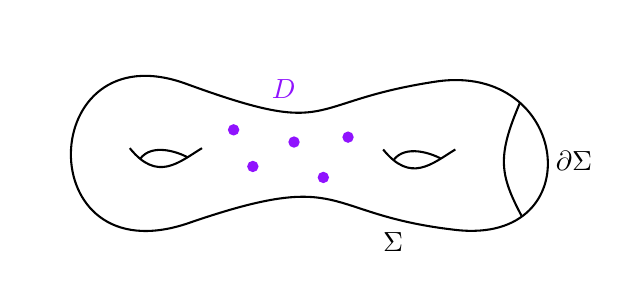
\begin{tikzpicture}[x=0.75pt,y=0.75pt,yscale=-1,xscale=1]

%Shape: Polygon Curved [id:ds035604419620915095] 
\draw   (79.37,25.97) .. controls (152.1,52.53) and (134.73,34.72) .. (199.52,24.9) .. controls (264.3,15.09) and (274.94,103.85) .. (209.22,96.35) .. controls (143.5,88.85) and (157.79,66.44) .. (80.63,93.01) .. controls (3.47,119.57) and (6.64,-0.59) .. (79.37,25.97) -- cycle ;
%Curve Lines [id:da7635811371660339] 
\draw    (52.17,56.96) .. controls (65.45,73.4) and (75.57,63.91) .. (86.95,56.96) ;
%Curve Lines [id:da8989271131706713] 
\draw    (57.23,62.02) .. controls (62.92,54.43) and (75.57,58.86) .. (80,61.39) ;
%Curve Lines [id:da5953645395125455] 
\draw    (174.23,57.59) .. controls (187.51,74.03) and (197.63,64.55) .. (209.01,57.59) ;
%Curve Lines [id:da4209585290119977] 
\draw    (179.29,62.65) .. controls (184.98,55.06) and (197.63,59.49) .. (202.06,62.02) ;
%Shape: Circle [id:dp3791131464091231] 
\draw  [color={rgb, 255:red, 144; green, 19; blue, 254 }  ,draw opacity=1 ][fill={rgb, 255:red, 144; green, 19; blue, 254 }  ,fill opacity=1 ] (99.98,48.13) .. controls (99.98,46.91) and (100.97,45.92) .. (102.19,45.92) .. controls (103.41,45.92) and (104.4,46.91) .. (104.4,48.13) .. controls (104.4,49.35) and (103.41,50.34) .. (102.19,50.34) .. controls (100.97,50.34) and (99.98,49.35) .. (99.98,48.13) -- cycle ;
%Shape: Ellipse [id:dp2374463332947847] 
\draw  [color={rgb, 255:red, 144; green, 19; blue, 254 }  ,draw opacity=1 ][fill={rgb, 255:red, 144; green, 19; blue, 254 }  ,fill opacity=1 ] (109.25,65.77) .. controls (109.25,64.55) and (110.23,63.57) .. (111.45,63.57) .. controls (112.67,63.57) and (113.66,64.55) .. (113.66,65.77) .. controls (113.66,66.99) and (112.67,67.98) .. (111.45,67.98) .. controls (110.23,67.98) and (109.25,66.99) .. (109.25,65.77) -- cycle ;
%Shape: Ellipse [id:dp35368836266522163] 
\draw  [color={rgb, 255:red, 144; green, 19; blue, 254 }  ,draw opacity=1 ][fill={rgb, 255:red, 144; green, 19; blue, 254 }  ,fill opacity=1 ] (129.09,54.01) .. controls (129.09,52.79) and (130.08,51.81) .. (131.3,51.81) .. controls (132.52,51.81) and (133.5,52.79) .. (133.5,54.01) .. controls (133.5,55.23) and (132.52,56.22) .. (131.3,56.22) .. controls (130.08,56.22) and (129.09,55.23) .. (129.09,54.01) -- cycle ;
%Shape: Ellipse [id:dp5744037578373786] 
\draw  [color={rgb, 255:red, 144; green, 19; blue, 254 }  ,draw opacity=1 ][fill={rgb, 255:red, 144; green, 19; blue, 254 }  ,fill opacity=1 ] (155.12,51.66) .. controls (155.12,50.44) and (156.1,49.45) .. (157.32,49.45) .. controls (158.54,49.45) and (159.53,50.44) .. (159.53,51.66) .. controls (159.53,52.88) and (158.54,53.86) .. (157.32,53.86) .. controls (156.1,53.86) and (155.12,52.88) .. (155.12,51.66) -- cycle ;
%Curve Lines [id:da3379921461483819] 
\draw    (240.29,34.8) .. controls (229.12,60.68) and (230.29,69.5) .. (240.88,89.49) ;
%Shape: Circle [id:dp9682521532873674] 
\draw  [color={rgb, 255:red, 144; green, 19; blue, 254 }  ,draw opacity=1 ][fill={rgb, 255:red, 144; green, 19; blue, 254 }  ,fill opacity=1 ] (143.21,71.07) .. controls (143.21,69.85) and (144.2,68.86) .. (145.41,68.86) .. controls (146.63,68.86) and (147.62,69.85) .. (147.62,71.07) .. controls (147.62,72.28) and (146.63,73.27) .. (145.41,73.27) .. controls (144.2,73.27) and (143.21,72.28) .. (143.21,71.07) -- cycle ;

% Text Node
\draw (172.73,96.1) node [anchor=north west][inner sep=0.75pt]    {$\Sigma $};
% Text Node
\draw (255.91,56.85) node [anchor=north west][inner sep=0.75pt]    {$\partial \Sigma $};
% Text Node
\draw (119.18,22.22) node [anchor=north west][inner sep=0.75pt]  [color={rgb, 255:red, 144; green, 19; blue, 254 }  ,opacity=1 ]  {$D$};
\end{tikzpicture}
\eea

Let $p\in D$ and $z$ be a local coordinate centered at $p$. Then locally $\omega$ can be written as
\bea \omega=\frac{\eta}{z^n}\eea
where $\eta$ is smooth, and $n\in \bZ$.
Since the pole order can be arbitrarily large, the naive $\int_\Sigma\omega$ is divergent in general. One intrinsic way out of this divergence problem \cite{Li:2020ljm} is as follows.
We can decompose $\omega$ into
\bea \omega=\alpha+\p\beta,\eea
where $\alpha$ is a 2-form with at most \emph{logarithmic pole} along $D$, $\beta$ is a $(0,1)$-form with \emph{arbitrary order of poles} along $D$, and $\p=dz\frac{\p}{\p z}$ is the holomorphic de Rham differential. 

\begin{rmk}
Such a decomposition \emph{exists} and is \emph{not unique}.
\end{rmk}

\begin{defn}[L-Zhou \cite{Li:2020ljm}]
Define the \textbf{regularized integral} 
\bea\dint_\Sigma\omega\coloneqq\int_\Sigma\alpha+\int_{\p\Sigma}\beta\eea
as a recipe to integrate the singular form $\omega$ on $\Sigma$, such that
\begin{itemize}
    \item it does NOT depend on the choice of $\alpha,\beta$,
    \item $\dint_\Sigma$ is invariant under conformal transformations,
    \item $\dint_\Sigma\p(-)=\int_{\p\Sigma}(-)$, 
    \item $\dint_\Sigma\pb(-)=\on{Res}(-)$.
\end{itemize}
\end{defn}
The regularized integral extends the usual integral for smooth forms, i.e., the following diagram is commutative:
\bea \begin{tikzcd}
\cA^2(\Sigma) \ar[rr, hook] \ar[dr, swap, "\int_\Sigma"]
&  & \cA^2(\Sigma,\star D) \ar[dl, "\dint_\Sigma"]\\
& \bC & 
\end{tikzcd}\eea

We can use this to define integrals on configuration space of $\Sigma$
\bea \on{Conf}_n(\Sigma)=\Sigma^n-\Delta =\lcb\left. (p_1,\cdots,p_n)\in\Sigma^n \right| p_i \neq p_j, \forall i\neq j\rcb\eea
and define
\bea\dint_{\Sigma^n} : \cA^{2n}(\Sigma^n,\star\Delta)\to \bC\eea
by
\bea \dint_{\Sigma^n}(-)= \dint_{\Sigma_1}\dint_{\Sigma_2}\cdots\ \dint_{\Sigma_n}(-).\eea
It does NOT depend on the choice of the ordering of the factors in $\Sigma^n$; Fubini-type theorem holds.
This gives an intrinsically regularized meaning for $\dint_{\Sigma^n} \Omega$, where $\Omega$ is the Feynman diagram integrand. 
This explains why the theory is UV finite.

\subsection{Homological structure of BV quantization}
Roughly speaking, BV quantization in QFT leads to \begin{itemize}
    \item factorization algebra $\on{Obs}$ of observables  \cite{costello2021factorization},
    \item a chain complex $\lb C_\blt(\on{Obs}),d\rb$ via algebraic structure of $\on{Obs}$,
    \item a BV algebra $\lb \cA,\Delta\rb$ describing the zero modes (at $L=\infty$) with a BV integration map
    \bea \int_{BV}: \cA\to \bC,\eea
    \item a $\bC[[\hbar]]$-linear map
    \bea \lan -\ran: C_\blt(\on{Obs})\to \cA((\hbar))\eea
    which is the HRG flow from $L=0$ to $L=\infty$ satisfying the QME $(d+\hbar\Delta)\lan -\ran=0$; the QME says that $\lan -\ran$ is a chain map intertwining $d$ and $\hbar\Delta$,
    \item partition function leading to the index theorem 
    \bea \on{Index}=\int_{BV}\lan 1\ran.\eea
\end{itemize}

Recall in the example of TQM,
we have the following data.
\begin{itemize}
    \item The factorization algebra is the Weyl algebra: $\on{Obs}=\cW_{2n}$.
    \item The factorization complex is the Hochschild chain complex $\lb C_\blt(\on{Obs}),d\rb$.
    \item BV algebra on zero modes: $\lb\cA,\Delta\rb=\lb \Omega^\blt(\bR^{2n}),\cL_{\omega^{-1}}\rb.$
    \item Free correlation map 
    \bea \lan -\ran: C_{\blt}(\cW_{2n})\to \Omega^\blt(\bR^{2n})((\hbar)), \quad b\mapsto \hbar \cL_{\omega^{-1}}.\eea
    \item $\on{Index}=\int_{BV}\lan 1\ran=\lsb e^{\omega_\hbar/\hbar}\widehat{A}\rsb$.
\end{itemize}
In the example of a 2d chiral QFT, we will have a similar story. \textsc{References}:
\cite{Gui:2021dci}.

\subsection{Beilinson-Drinfeld's chiral chain complex}
Intuitively, chiral chain complex can be viewed as a 2d chiral analogue of Hochschild chain complex.
\bea 
\tikzset{every picture/.style={line width=0.75pt}}
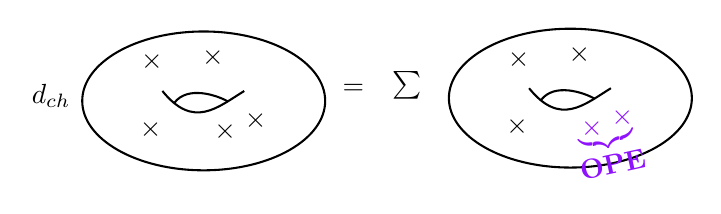
\begin{tikzpicture}[x=0.75pt,y=0.75pt,yscale=-1,xscale=1]

%Curve Lines [id:da635337608272412] 
\draw    (99.3,113.01) .. controls (114.35,131.65) and (125.82,120.89) .. (138.73,113.01) ;
%Curve Lines [id:da011829695865262835] 
\draw    (105.03,118.74) .. controls (111.49,110.14) and (125.82,115.16) .. (130.84,118.03) ;
%Shape: Ellipse [id:dp6950451999185667] 
\draw   (60.67,117.78) .. controls (60.67,99.31) and (86.87,84.33) .. (119.19,84.33) .. controls (151.52,84.33) and (177.72,99.31) .. (177.72,117.78) .. controls (177.72,136.25) and (151.52,151.22) .. (119.19,151.22) .. controls (86.87,151.22) and (60.67,136.25) .. (60.67,117.78) -- cycle ;
%Curve Lines [id:da5951843766986344] 
\draw    (275.96,111.67) .. controls (291.02,130.31) and (302.49,119.56) .. (315.4,111.67) ;
%Curve Lines [id:da849863385797317] 
\draw    (281.7,117.41) .. controls (288.15,108.81) and (302.49,113.82) .. (307.51,116.69) ;
%Shape: Ellipse [id:dp5521894453900986] 
\draw   (237.33,116.44) .. controls (237.33,97.97) and (263.54,83) .. (295.86,83) .. controls (328.19,83) and (354.39,97.97) .. (354.39,116.44) .. controls (354.39,134.92) and (328.19,149.89) .. (295.86,149.89) .. controls (263.54,149.89) and (237.33,134.92) .. (237.33,116.44) -- cycle ;

% Text Node
\draw (87.56,93.07) node [anchor=north west][inner sep=0.75pt]    {$\times $};
% Text Node
\draw (116.89,91.07) node [anchor=north west][inner sep=0.75pt]    {$\times $};
% Text Node
\draw (86.89,125.73) node [anchor=north west][inner sep=0.75pt]    {$\times $};
% Text Node
\draw (122.89,126.4) node [anchor=north west][inner sep=0.75pt]    {$\times $};
% Text Node
\draw (137.51,121.43) node [anchor=north west][inner sep=0.75pt]    {$\times $};
% Text Node
\draw (34.89,108.07) node [anchor=north west][inner sep=0.75pt]    {$d_{ch}$};
% Text Node
\draw (264.22,91.73) node [anchor=north west][inner sep=0.75pt]    {$\times $};
% Text Node
\draw (293.56,89.73) node [anchor=north west][inner sep=0.75pt]    {$\times $};
% Text Node
\draw (263.56,124.4) node [anchor=north west][inner sep=0.75pt]    {$\times $};
% Text Node
\draw (299.56,125.07) node [anchor=north west][inner sep=0.75pt]  [color={rgb, 255:red, 144; green, 19; blue, 254 }  ,opacity=1 ]  {$\times $};
% Text Node
\draw (314.18,120.09) node [anchor=north west][inner sep=0.75pt]  [color={rgb, 255:red, 144; green, 19; blue, 254 }  ,opacity=1 ]  {$\times $};
% Text Node
\draw (184.67,108.07) node [anchor=north west][inner sep=0.75pt]    {$=$};
% Text Node
\draw (208.67,102.07) node [anchor=north west][inner sep=0.75pt]    {$\sum $};
% Text Node
\draw (295.31,134.74) node [anchor=north west][inner sep=0.75pt]  [color={rgb, 255:red, 144; green, 19; blue, 254 }  ,opacity=1 ,rotate=-347.56]  {$\underbrace{\ \ \ \ \ \ }_{\textbf{OPE}}$};
\end{tikzpicture}
\eea

\begin{itemize}
    \item \cite{zhu1994global} studies the space of genus 1 conformal blocks (i.e. the 0th elliptic chiral homology).
    \item \cite{beilinson2004chiral} explores the chiral homology for general algebraic curves.
    \item \cite{van2021chiral,van2021first} constructed explicit complexes expressing the 0th and 1st elliptic chiral homology.
\end{itemize}

\paragraph{The construction of Beilinson-Drinfeld.}
Given the following data:
\begin{itemize}
    \item a category of right $\cD$-modules $\cM(X)$ on $X=\Sigma$,
    \item a category of right $\cD$-modules $\cM(X^S)$ on $X^S$, such that each element $M \in\cM(X^S)$ is a collection that assigns every finite index set $I\in S$ a right $\cD$-module $\cM_{X^I}$ on the product $X^I$ satisfying certain compatibility conditions,
    \item there is an exact fully faithful embedding
    \bea \Delta^{(S)}_\star: \cM(X)\hookrightarrow \cM(X^S)\eea
    via the diagonal map $\Delta^{(I)}:X \hookrightarrow X^I$,
    \item $\cM(X^S)$ carries a (chiral) tensor structure $\otimes^{ch}$,
\end{itemize}
then a chiral algebra $\cA$ is a \textbf{Lie algebraic object} via $\Delta^{(S)}_\star$. 

\begin{rmk}
The chiral algebra $\cA$ collects all ``normal ordering operators.''
\end{rmk}

We consider the Chevalley-Eilenberg (CE) complex
\bea \lb C(\cA),d_{CE}\rb=\lb \bigoplus_{\blt>0} \sym^\blt_{\otimes^{ch}}\lb \Delta^{(S)}_\star\cA[1]\rb, d_{CE}\rb.\eea
The chiral homology for this complex is
\bea C^{ch}(X,\cA)=R\Gamma_{DR}(X^S, C(\cA)).\eea

We will focus on $\beta\gamma-bc$ system, where the vertex operator algebra (VOA) $\cV^{\beta\gamma-bc}$ is the chiral algebra $\cA^{\beta\gamma-bc}$.
\begin{thm}[Gui-L \cite{Gui:2021dci}]
Let $E$ be an elliptic curve. Then the HRG flow gives a map
\bea \lan -\ran_{2d}: C^{ch}(E,\cA^{\beta\gamma-bc})\to \cA((\hbar))\eea
satisfying the QME $(d_{ch}+\hbar\Delta)\lan -\ran_{2d}=0$.
Roughly speaking, $\lan -\ran$ is defined by
\bea \lan \cO_1\otimes\cdots\otimes\cO_n\ran_{2d}\coloneqq \dint_{E^n} \lan \cO_1(z_1)\cdots \cO_n(z_n) \ran\eea
where $\lan \cO_1(z_1)\cdots \cO_n(z_n) \ran$
is a local correlator given by the Feynman diagram, and $\dint_{E^n}$ is the regularized integral.
\end{thm}


\subsection{2d $\to$ 1d reduction}
We summarize our discussion as follows.
\begin{table}[!htpb]\centering
            \begin{tabular}{c|c}\toprule
            \textbf{1d TQM} & \textbf{2d chiral QFT}\\ \hline
            Associative algebra & Vertex/chiral algebra\\ \hline
            Hochschild homology & Chiral homology\\ \hline 
            QME $(\hbar\Delta+b)\lan -\ran_{1d}=0$ & QME $(\hbar\Delta+d_{ch})\lan -\ran_{2d}=0$ \\ \hline
            $\lan \cO_1\otimes\cdots\otimes\cO_n\ran_{1d}=\int_{\ols{\on{Conf}_n(S^1)}}$ & $\lan \cO_1\otimes\cdots\otimes\cO_n\ran_{2d}=\dint_{\Sigma^n}$ \\ 
            \bottomrule
            \end{tabular}
\end{table}

In physics, the partition functions/correlation functions on elliptic curves are described by QM on $S^1$.
\bea 
\tikzset{every picture/.style={line width=0.75pt}}       
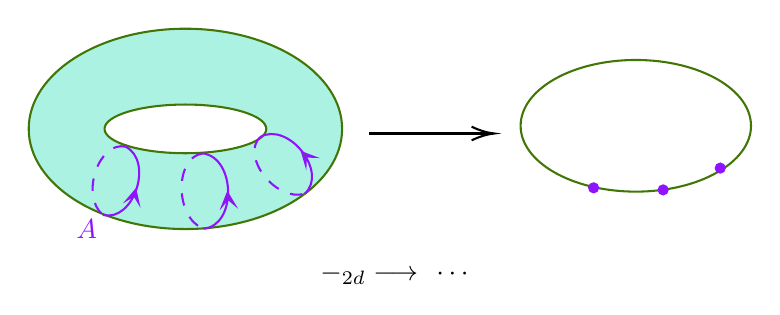
\begin{tikzpicture}[x=0.75pt,y=0.75pt,yscale=-1,xscale=1]

%Shape: Ellipse [id:dp4418092526097801] 
\draw  [color={rgb, 255:red, 65; green, 117; blue, 5 }  ,draw opacity=1 ] (321.5,63.79) .. controls (321.5,46.27) and (346.35,32.07) .. (377,32.07) .. controls (407.65,32.07) and (432.5,46.27) .. (432.5,63.79) .. controls (432.5,81.3) and (407.65,95.5) .. (377,95.5) .. controls (346.35,95.5) and (321.5,81.3) .. (321.5,63.79) -- cycle ;
%Straight Lines [id:da6931809500773398] 
\draw    (248.5,67.5) -- (306.83,67.5) ;
\draw [shift={(308.83,67.5)}, rotate = 180] [color={rgb, 255:red, 0; green, 0; blue, 0 }  ][line width=0.75]    (10.93,-3.29) .. controls (6.95,-1.4) and (3.31,-0.3) .. (0,0) .. controls (3.31,0.3) and (6.95,1.4) .. (10.93,3.29)   ;
%Shape: Circle [id:dp9584222087677268] 
\draw  [color={rgb, 255:red, 144; green, 19; blue, 254 }  ,draw opacity=1 ][fill={rgb, 255:red, 144; green, 19; blue, 254 }  ,fill opacity=1 ] (354.5,93.67) .. controls (354.5,92.47) and (355.47,91.5) .. (356.67,91.5) .. controls (357.86,91.5) and (358.83,92.47) .. (358.83,93.67) .. controls (358.83,94.86) and (357.86,95.83) .. (356.67,95.83) .. controls (355.47,95.83) and (354.5,94.86) .. (354.5,93.67) -- cycle ;
%Shape: Circle [id:dp8524982473210796] 
\draw  [color={rgb, 255:red, 144; green, 19; blue, 254 }  ,draw opacity=1 ][fill={rgb, 255:red, 144; green, 19; blue, 254 }  ,fill opacity=1 ] (388,94.67) .. controls (388,93.47) and (388.97,92.5) .. (390.17,92.5) .. controls (391.36,92.5) and (392.33,93.47) .. (392.33,94.67) .. controls (392.33,95.86) and (391.36,96.83) .. (390.17,96.83) .. controls (388.97,96.83) and (388,95.86) .. (388,94.67) -- cycle ;
%Shape: Circle [id:dp1755796687587492] 
\draw  [color={rgb, 255:red, 144; green, 19; blue, 254 }  ,draw opacity=1 ][fill={rgb, 255:red, 144; green, 19; blue, 254 }  ,fill opacity=1 ] (415.5,84.17) .. controls (415.5,82.97) and (416.47,82) .. (417.67,82) .. controls (418.86,82) and (419.83,82.97) .. (419.83,84.17) .. controls (419.83,85.36) and (418.86,86.33) .. (417.67,86.33) .. controls (416.47,86.33) and (415.5,85.36) .. (415.5,84.17) -- cycle ;
%Shape: Donut [id:dp07063864397558173] 
\draw  [color={rgb, 255:red, 65; green, 117; blue, 5 }  ,draw opacity=1 ][fill={rgb, 255:red, 80; green, 227; blue, 194 }  ,fill opacity=0.48 ,even odd rule] (121.03,65.26) .. controls (121.03,58.79) and (138.48,53.54) .. (160,53.54) .. controls (181.52,53.55) and (198.96,58.8) .. (198.96,65.28) .. controls (198.96,71.75) and (181.52,77) .. (160,77) .. controls (138.48,76.99) and (121.03,71.74) .. (121.03,65.26)(84.5,65.26) .. controls (84.51,38.61) and (118.31,17.01) .. (160.01,17.01) .. controls (201.7,17.02) and (235.5,38.63) .. (235.49,65.28) .. controls (235.49,91.93) and (201.68,113.53) .. (159.99,113.53) .. controls (118.29,113.52) and (84.5,91.91) .. (84.5,65.26) ;
%Curve Lines [id:da0009892278601366655] 
\draw [color={rgb, 255:red, 144; green, 19; blue, 254 }  ,draw opacity=1 ]   (196,69.19) .. controls (209.5,61.53) and (229,86.03) .. (217.5,96.53) ;
%Curve Lines [id:da44799976092621097] 
\draw [color={rgb, 255:red, 144; green, 19; blue, 254 }  ,draw opacity=1 ] [dash pattern={on 4.5pt off 4.5pt}]  (196,69.19) .. controls (186.5,78.53) and (203.5,100.53) .. (217.5,96.53) ;
\draw  [color={rgb, 255:red, 144; green, 19; blue, 254 }  ,draw opacity=1 ][fill={rgb, 255:red, 65; green, 117; blue, 5 }  ,fill opacity=1 ] (217.89,82.25) -- (216.27,76.66) -- (221.72,78.72) -- (218.04,78.57) -- cycle ;
%Curve Lines [id:da04657738471784345] 
\draw [color={rgb, 255:red, 144; green, 19; blue, 254 }  ,draw opacity=1 ]   (168.5,77.07) .. controls (184.43,79.43) and (184.7,112.12) .. (168.59,113.38) ;
%Curve Lines [id:da24828006383038592] 
\draw [color={rgb, 255:red, 144; green, 19; blue, 254 }  ,draw opacity=1 ] [dash pattern={on 4.5pt off 4.5pt}]  (168.5,77.07) .. controls (154.77,78.65) and (154.6,107.68) .. (168.59,113.38) ;
\draw  [color={rgb, 255:red, 144; green, 19; blue, 254 }  ,draw opacity=1 ][fill={rgb, 255:red, 65; green, 117; blue, 5 }  ,fill opacity=1 ] (178.04,101.88) -- (180.29,96.23) -- (183.42,101.43) -- (180.51,98.94) -- cycle ;
%Curve Lines [id:da43201889595924503] 
\draw [color={rgb, 255:red, 144; green, 19; blue, 254 }  ,draw opacity=1 ]   (131.17,73.82) .. controls (144.86,80.83) and (135.11,110.48) .. (120.16,106.69) ;
%Curve Lines [id:da5919508883701639] 
\draw [color={rgb, 255:red, 144; green, 19; blue, 254 }  ,draw opacity=1 ] [dash pattern={on 4.5pt off 4.5pt}]  (131.17,73.82) .. controls (118.27,71.06) and (109.24,97.26) .. (120.16,106.69) ;
\draw  [color={rgb, 255:red, 144; green, 19; blue, 254 }  ,draw opacity=1 ][fill={rgb, 255:red, 65; green, 117; blue, 5 }  ,fill opacity=1 ] (132.22,99.18) -- (135.98,94.76) -- (137.22,100.42) -- (135.35,97.28) -- cycle ;

% Text Node
\draw (223.5,128.9) node [anchor=north west][inner sep=0.75pt]    {$\lan - \ran_{2d} \longrightarrow \Tr_{\cH}\ \lan\cdots\ran$};
% Text Node
\draw (106,107.59) node [anchor=north west][inner sep=0.75pt]  [color={rgb, 255:red, 144; green, 19; blue, 254 }  ,opacity=1 ]  {$A$};
\end{tikzpicture}
\eea
Now we can define 2d correlation function using \emph{regularized integral} $\dint_E$. In 1d, operators are described by $A$-cycle $\oint_A$. These two integrals are not exactly the same, but related to each other by \emph{holomorphic anomaly}.

\begin{thm}[L-Zhou \cite{Li:2020ljm}]
Let $\Phi(z_1,\cdots,z_n;\tau)$ be a meromorphic elliptic function on $\bC^n\times \bH$ which is holomorphic away from diagonals. Let $A_1,\cdots,A_n$ be $n$ disjoint $A$-cycles on the elliptic curve $E_\tau=\bC/(\bZ\oplus \tau\bZ)$. 
\bea 
\tikzset{every picture/.style={line width=0.75pt}} 
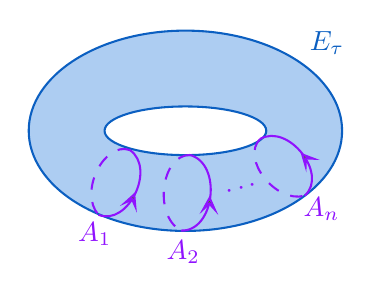
\begin{tikzpicture}[x=0.75pt,y=0.75pt,yscale=-1,xscale=1]
%Shape: Donut [id:dp6629776521166959] 
\draw  [color={rgb, 255:red, 11; green, 95; blue, 193 }  ,draw opacity=1 ][fill={rgb, 255:red, 74; green, 144; blue, 226 }  ,fill opacity=0.45 ,even odd rule] (244.53,97.57) .. controls (244.53,91.09) and (261.98,85.84) .. (283.5,85.85) .. controls (305.02,85.85) and (322.46,91.11) .. (322.46,97.58) .. controls (322.46,104.06) and (305.02,109.31) .. (283.5,109.3) .. controls (261.98,109.3) and (244.53,104.05) .. (244.53,97.57)(208,97.56) .. controls (208.01,70.91) and (241.81,49.31) .. (283.51,49.32) .. controls (325.2,49.33) and (359,70.94) .. (358.99,97.59) .. controls (358.99,124.24) and (325.18,145.84) .. (283.49,145.83) .. controls (241.79,145.83) and (208,124.21) .. (208,97.56) ;
%Curve Lines [id:da724728305831202] 
\draw [color={rgb, 255:red, 144; green, 19; blue, 254 }  ,draw opacity=1 ]   (319.5,101.5) .. controls (333,93.83) and (352.5,118.33) .. (341,128.83) ;
%Curve Lines [id:da09375441458438294] 
\draw [color={rgb, 255:red, 144; green, 19; blue, 254 }  ,draw opacity=1 ] [dash pattern={on 4.5pt off 4.5pt}]  (319.5,101.5) .. controls (310,110.83) and (327,132.83) .. (341,128.83) ;
\draw  [color={rgb, 255:red, 144; green, 19; blue, 254 }  ,draw opacity=1 ][fill={rgb, 255:red, 65; green, 117; blue, 5 }  ,fill opacity=1 ] (341.39,114.56) -- (339.77,108.96) -- (345.22,111.03) -- (341.54,110.88) -- cycle ;
%Curve Lines [id:da3775426299589082] 
\draw [color={rgb, 255:red, 144; green, 19; blue, 254 }  ,draw opacity=1 ]   (285.75,109.23) .. controls (301.43,113.61) and (297.57,146.42) .. (281.26,145.65) ;
%Curve Lines [id:da43322948676756656] 
\draw [color={rgb, 255:red, 144; green, 19; blue, 254 }  ,draw opacity=1 ] [dash pattern={on 4.5pt off 4.5pt}]  (285.75,109.23) .. controls (271.79,109.09) and (267.95,138.17) .. (281.26,145.65) ;
\draw  [color={rgb, 255:red, 144; green, 19; blue, 254 }  ,draw opacity=1 ][fill={rgb, 255:red, 65; green, 117; blue, 5 }  ,fill opacity=1 ] (292.18,135.31) -- (295.16,129.94) -- (297.64,135.54) -- (295.04,132.68) -- cycle ;
%Curve Lines [id:da9527348448178135] 
\draw [color={rgb, 255:red, 144; green, 19; blue, 254 }  ,draw opacity=1 ]   (256.75,106.87) .. controls (269.43,115.57) and (255.96,143.72) .. (241.61,138.05) ;
%Curve Lines [id:da12633292871659774] 
\draw [color={rgb, 255:red, 144; green, 19; blue, 254 }  ,draw opacity=1 ] [dash pattern={on 4.5pt off 4.5pt}]  (256.75,106.87) .. controls (244.31,102.47) and (231.99,127.3) .. (241.61,138.05) ;
\draw  [color={rgb, 255:red, 144; green, 19; blue, 254 }  ,draw opacity=1 ][fill={rgb, 255:red, 65; green, 117; blue, 5 }  ,fill opacity=1 ] (254.53,132.14) -- (258.83,128.25) -- (259.34,134.02) -- (257.88,130.66) -- cycle ;

% Text Node
\draw (230.33,140.23) node [anchor=north west][inner sep=0.75pt]  [color={rgb, 255:red, 144; green, 19; blue, 254 }  ,opacity=1 ]  {$A_{1}$};
% Text Node
\draw (310.43,125.53) node  [color={rgb, 255:red, 144; green, 19; blue, 254 }  ,opacity=1 ,rotate=-346.47]  {$\cdots $};
% Text Node
\draw (339,128.4) node [anchor=north west][inner sep=0.75pt]  [color={rgb, 255:red, 144; green, 19; blue, 254 }  ,opacity=1 ]  {$A_{n}$};
% Text Node
\draw (273,148.9) node [anchor=north west][inner sep=0.75pt]  [color={rgb, 255:red, 144; green, 19; blue, 254 }  ,opacity=1 ]  {$A_{2}$};
% Text Node
\draw (342,48.4) node [anchor=north west][inner sep=0.75pt]  [color={rgb, 255:red, 11; green, 95; blue, 193 }  ,opacity=1 ]  {$E_{\tau }$};
\end{tikzpicture}
\eea
Then the regularized integral 
\bea\dint_{E^n_\tau}\lb \prod_{i=1}^n \frac{d^2z_i}{\Im \tau}\rb \Phi(z_1,\cdots,z_n;\tau)\eea
lies in $\sO_{\bH}\lsb\frac{1}{\Im \tau}\rsb$. Moreover, we have
\bea\lim_{\ols{\tau}\to\infty}\dint_{E^n_\tau} \lb \prod_{i=1}^n\frac{d^2z_i}{\Im \tau}\rb \Phi
=\frac{1}{n!}\sum_{\sigma\in S_n}\int_{A_{\sigma(1)}} dz_1 \cdots \int_{A_{\sigma(n)}} dz_n\ \Phi,\eea
where $S_n$ is the permutation group for $n$.
Essentially this means
\bea\dint_{E^n}\xrightarrow{\lim_{\ols{\tau}\to\infty}} \text{averaged } \int_A,\eea
where $\dint_{E^n}$ is almost holomorphic modular, whereas the averaged $\int_A$ is quasi-modular.
\end{thm}
The anti-holomorphic dependence has a precise description.

\begin{thm}[L-Zhou \cite{Li:2020ljm}]
Let $\Phi$ be an almost-elliptic function. Then one has 
\bea \p_Y\dint_{E^n_\tau}\Phi= \dint_{E^n_\tau}\p_Y\Phi
-\sum_{i<j} \dint_{E^{n-1}_\tau}\on{Res}_{z_i=z_j}\lb(z_i-z_j)\Phi\rb.\eea
Here $Y=\frac{1}{\Im \tau}$.
This gives the \textbf{holomorphic anomaly equation}.
\end{thm}

